\section{Adding a disturbance observer to an existing feedback controller}
\begin{frame}
    \frametitle{Outline}
    \tableofcontents[currentsection]
\end{frame}

\begin{frame}
    \frametitle{Adding a disturbance observer to an existing controller}

    Suppose we have designed a controller $C(z)$ for the interconnection
    \begin{figure}
        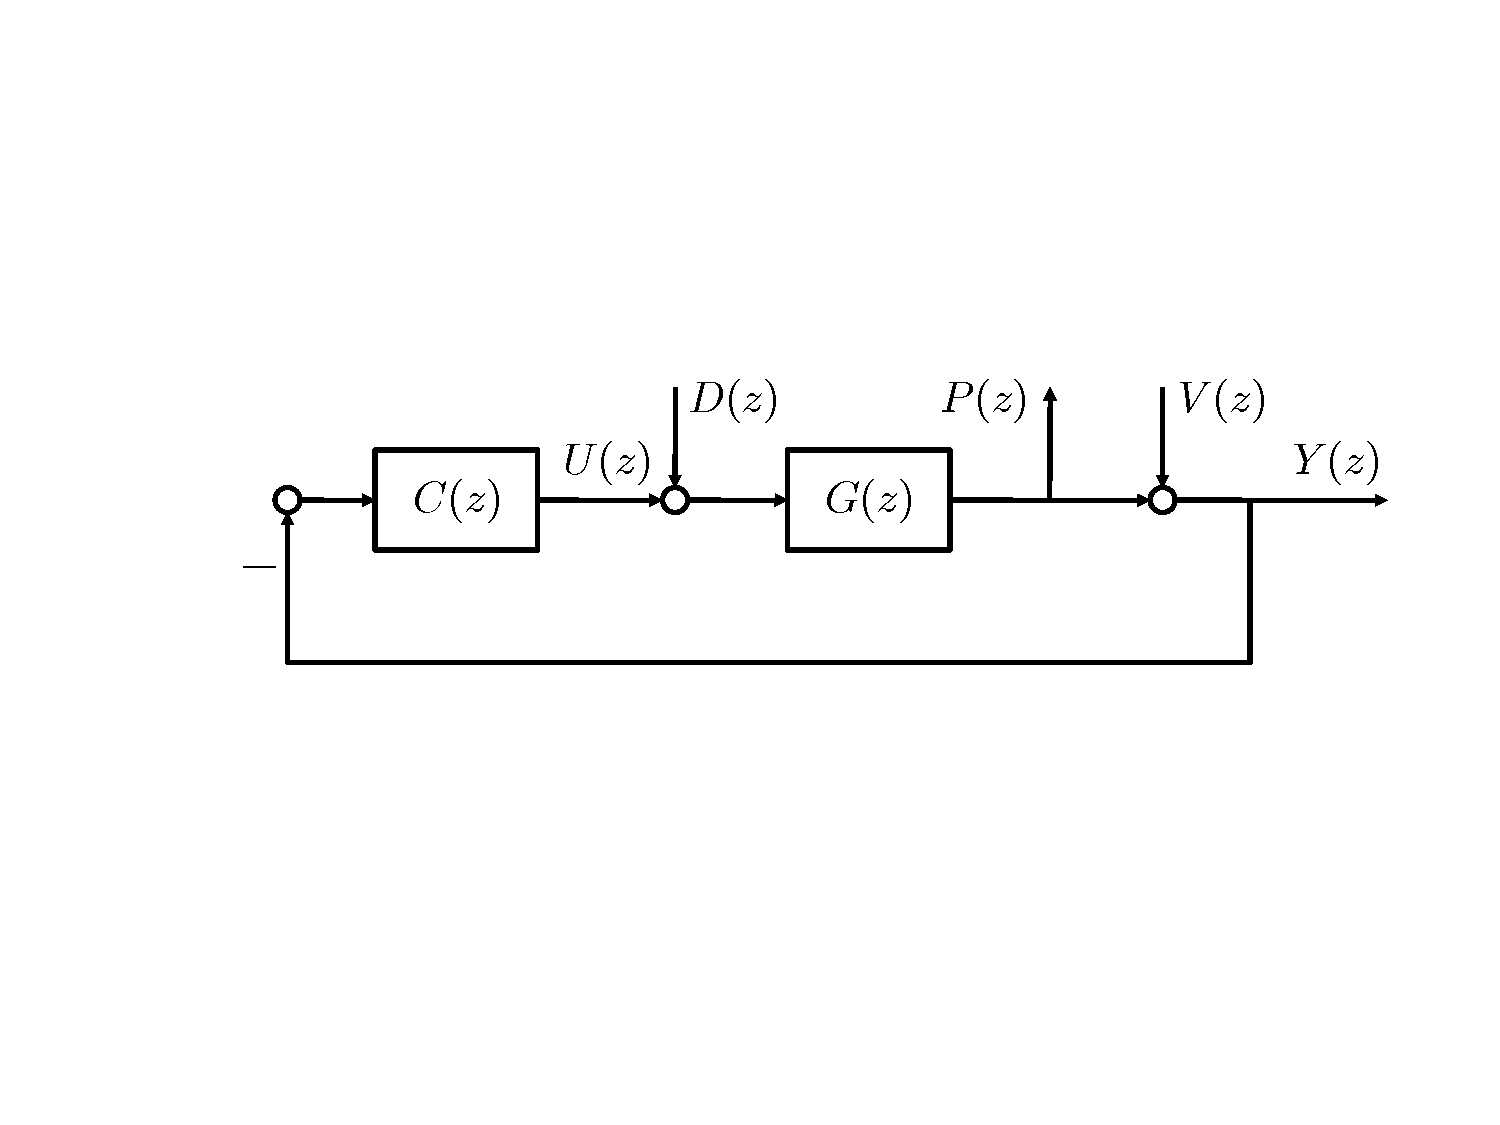
\includegraphics[width=0.5\textwidth]{Disturbance_Observer_multi1}
    \end{figure}
    and we would like to add a disturbance observer:
    \begin{figure}
        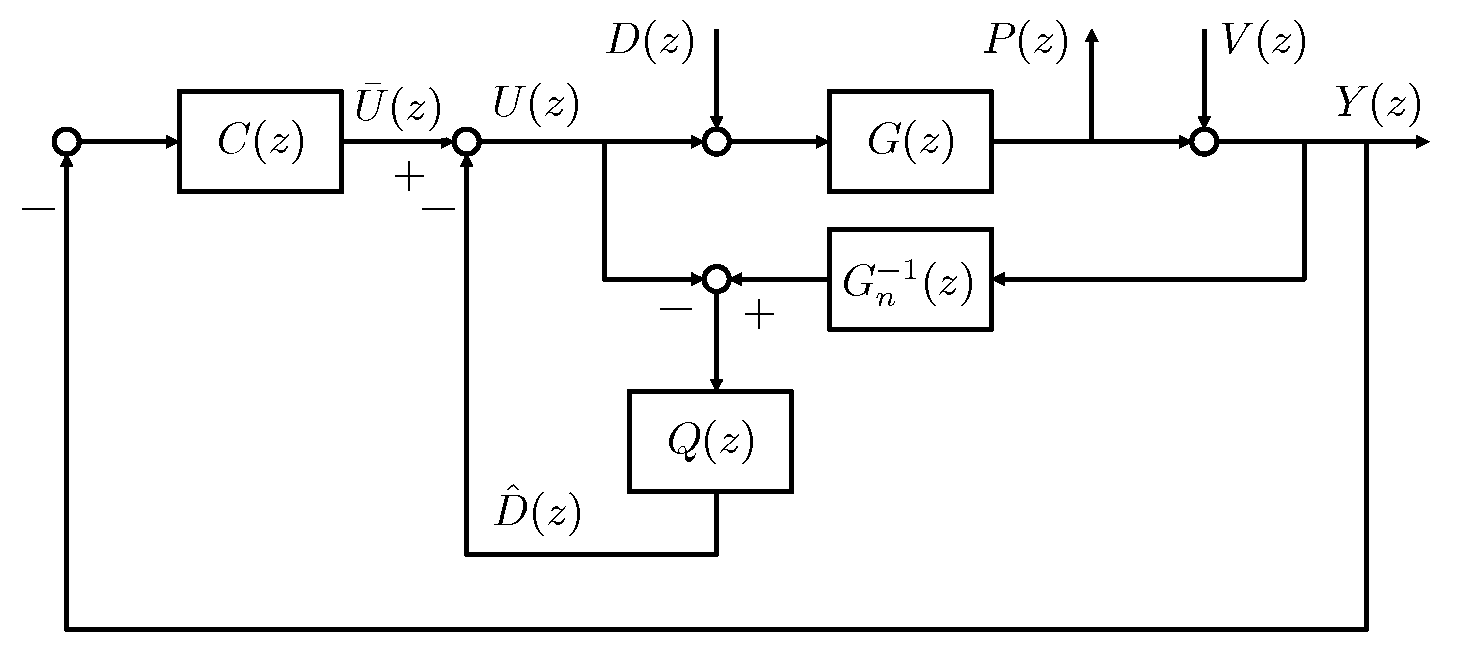
\includegraphics[width=0.5\textwidth]{Disturbance_Observer_multi2}
    \end{figure}
    \pause
    How does this affect the stability of the closed-loop system?

\end{frame}

\begin{frame}
    \frametitle{Adding a disturbance observer to an existing controller}

    \begin{figure}
        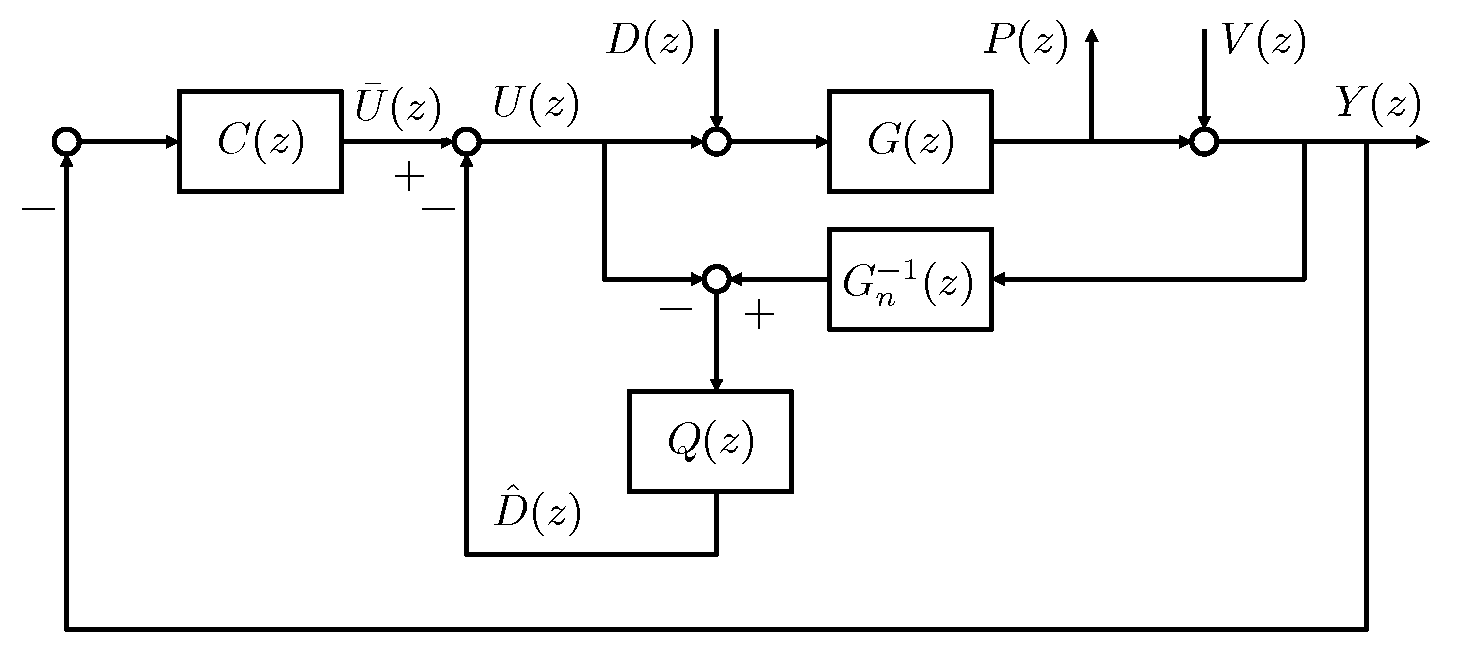
\includegraphics[width=0.4\textwidth]{Disturbance_Observer_multi2}
    \end{figure}
    Since we are only interested in stability, we set the exogenous inputs to zero. Also, we let $G(z) = G_n(z) ( 1 + \Delta(z))$.
    \pause
    \begin{figure}
        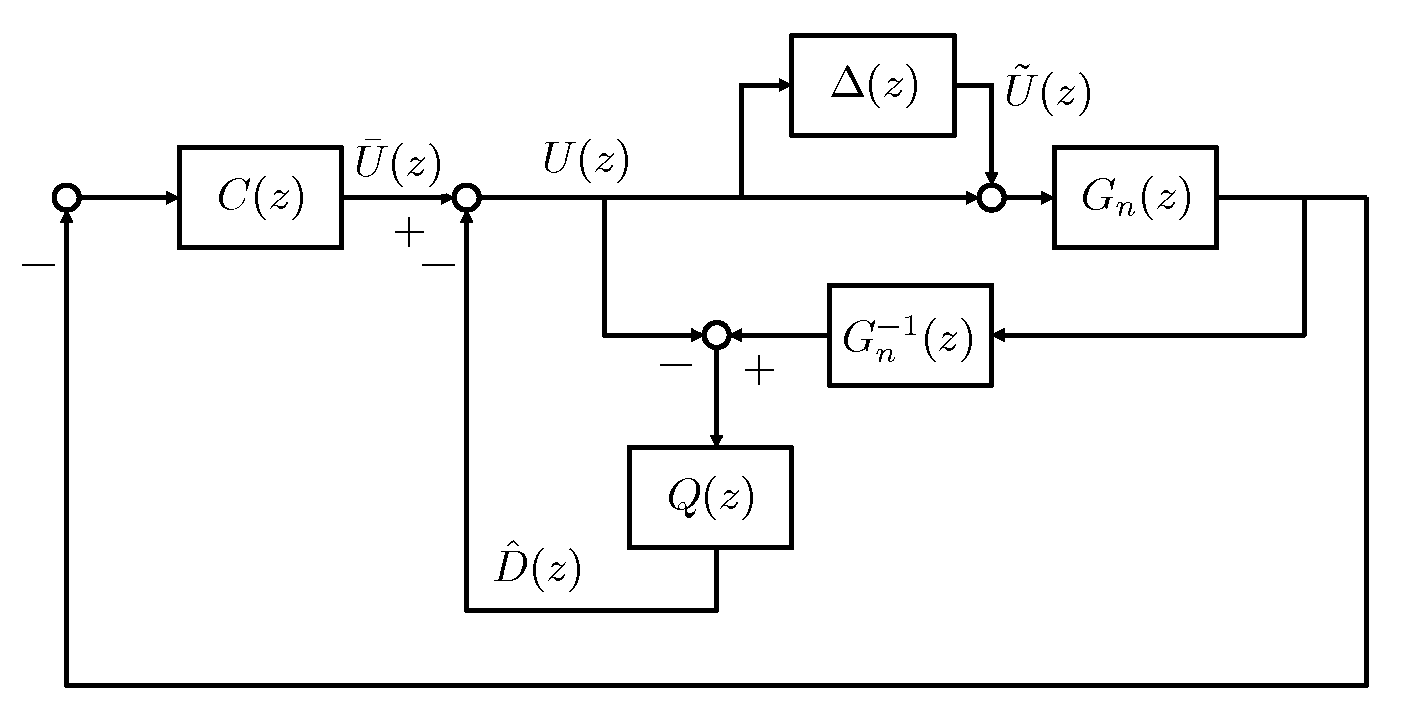
\includegraphics[width=0.5\textwidth]{Disturbance_Observer_multi3}
    \end{figure}
    \pause

    To use the small-gain theorem, we must simplify this to a feedback interconnection of $\Delta(z)$ and another system.

\end{frame}

\begin{frame}
    \frametitle{Simplifying the closed-loop representation}

    Removing $\Delta(z)$ from the interconnection, we have
    \begin{figure}
        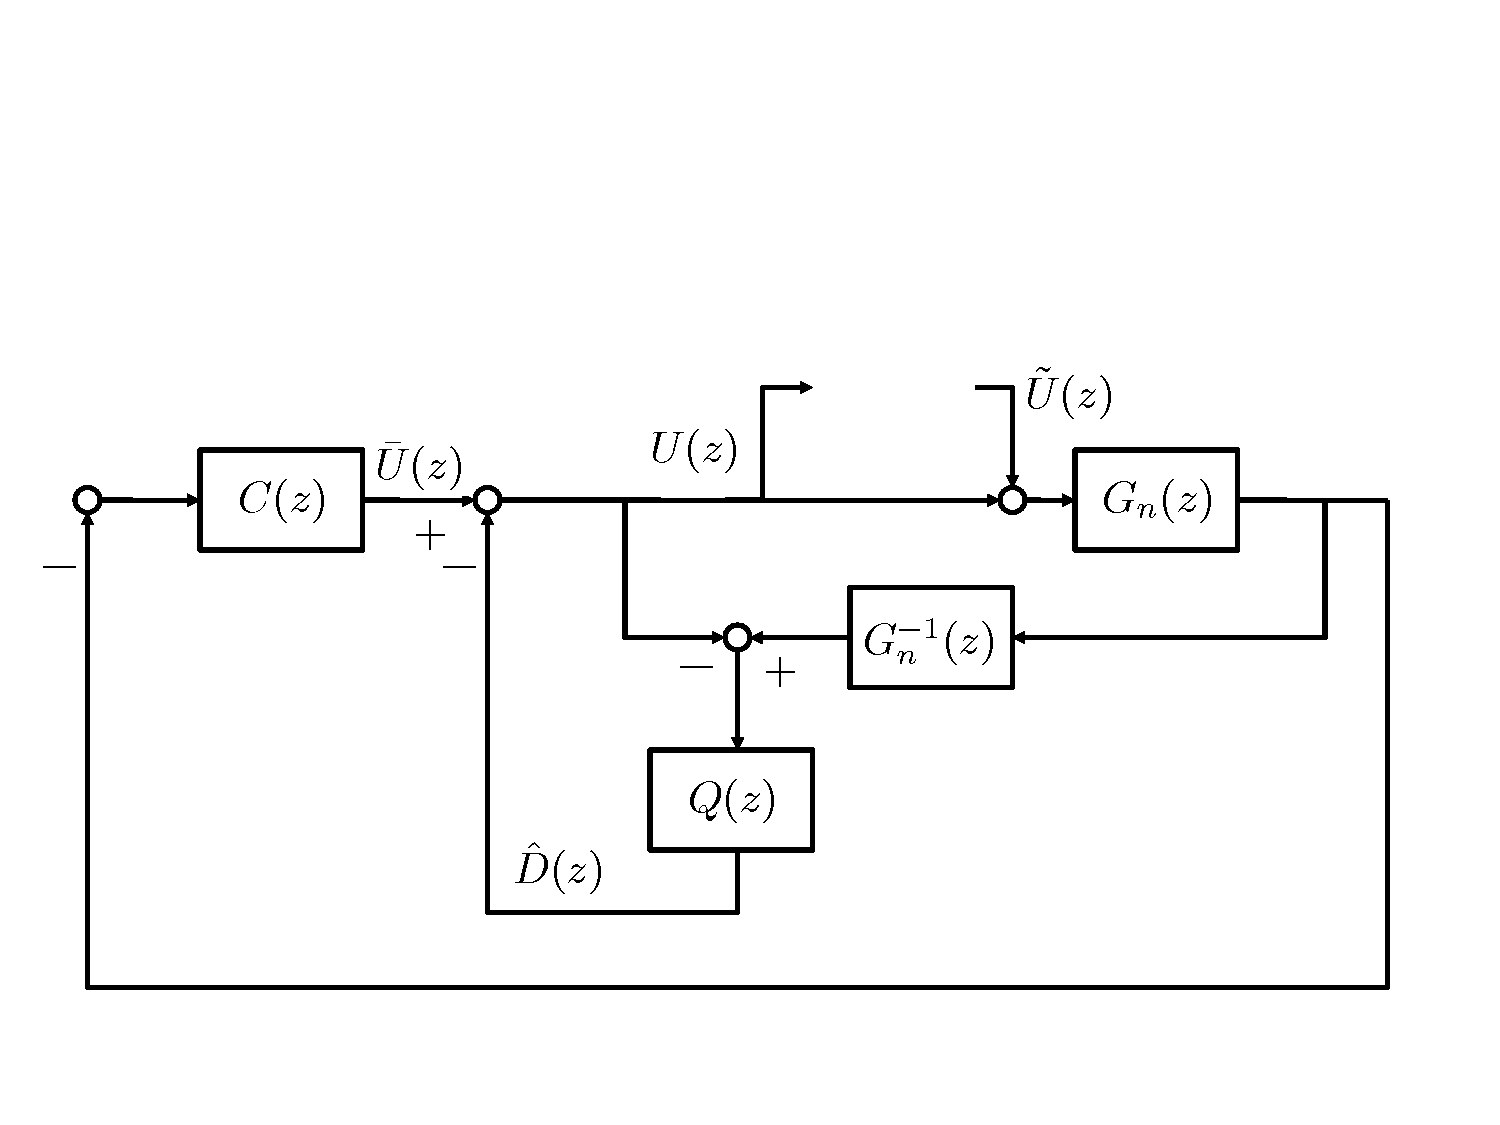
\includegraphics[width=0.5\textwidth]{Disturbance_Observer_multi4}
    \end{figure}
    \pause
    Omitting dependency on $z$, we have
    \begin{gather*}
        \hat{D} = Q \left[ \frac{G_n}{G_n}(\tilde{U} + U) - U \right]
            \quad \Rightarrow \quad \hat{D} = Q \tilde{U} \\
        U = -CG_n (\tilde{U} + U) - \hat{D}
            \quad \Rightarrow \quad U = -CG_n(\tilde{U} + U) - Q \tilde{U} \\
        \Rightarrow \quad (1 + CG_n) U = -(CG_n + Q) \tilde{U}
    \end{gather*}

\end{frame}

\begin{frame}
    \frametitle{Closed-loop stability}

    We now have the simplified closed-loop system representation
    \begin{figure}
        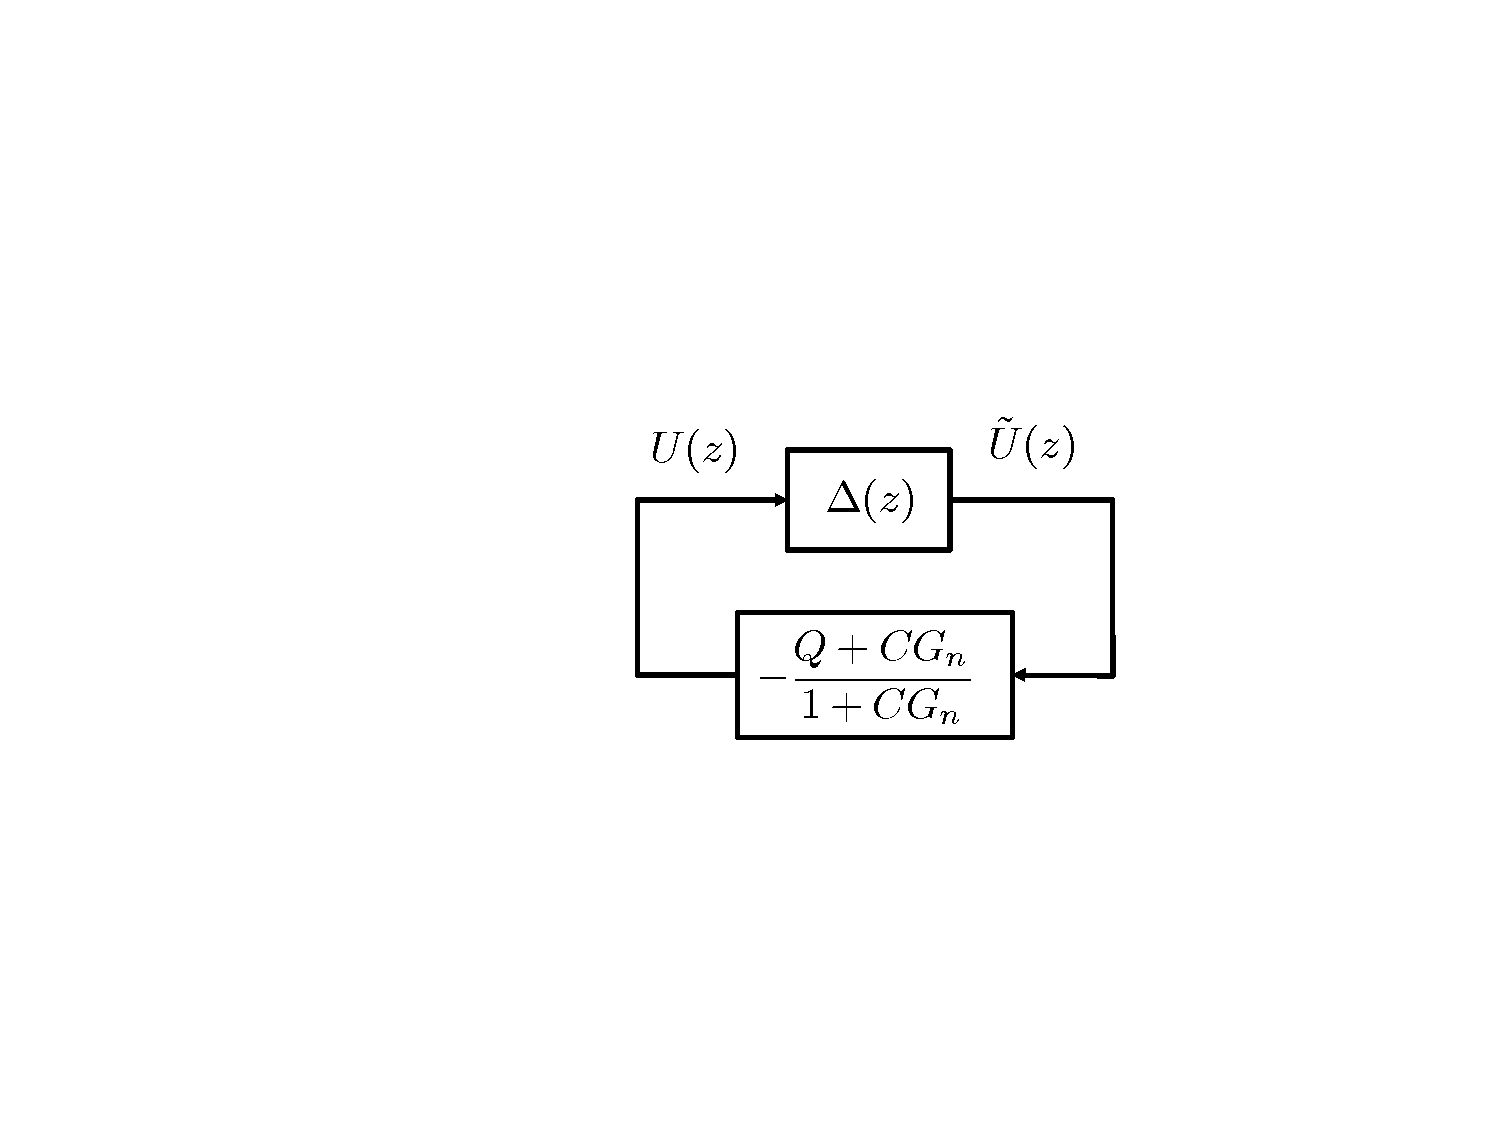
\includegraphics[width=0.3\textwidth]{Disturbance_Observer_multi5}
    \end{figure}
    \pause
    Using the small-gain theorem, we can therefore guarantee closed-loop stability if:
    \begin{enumerate}
    \item
    $G_n(z)$ is minimum phase
    \pause

    \item
    The following feedback interconnection is stable
    \begin{figure}
        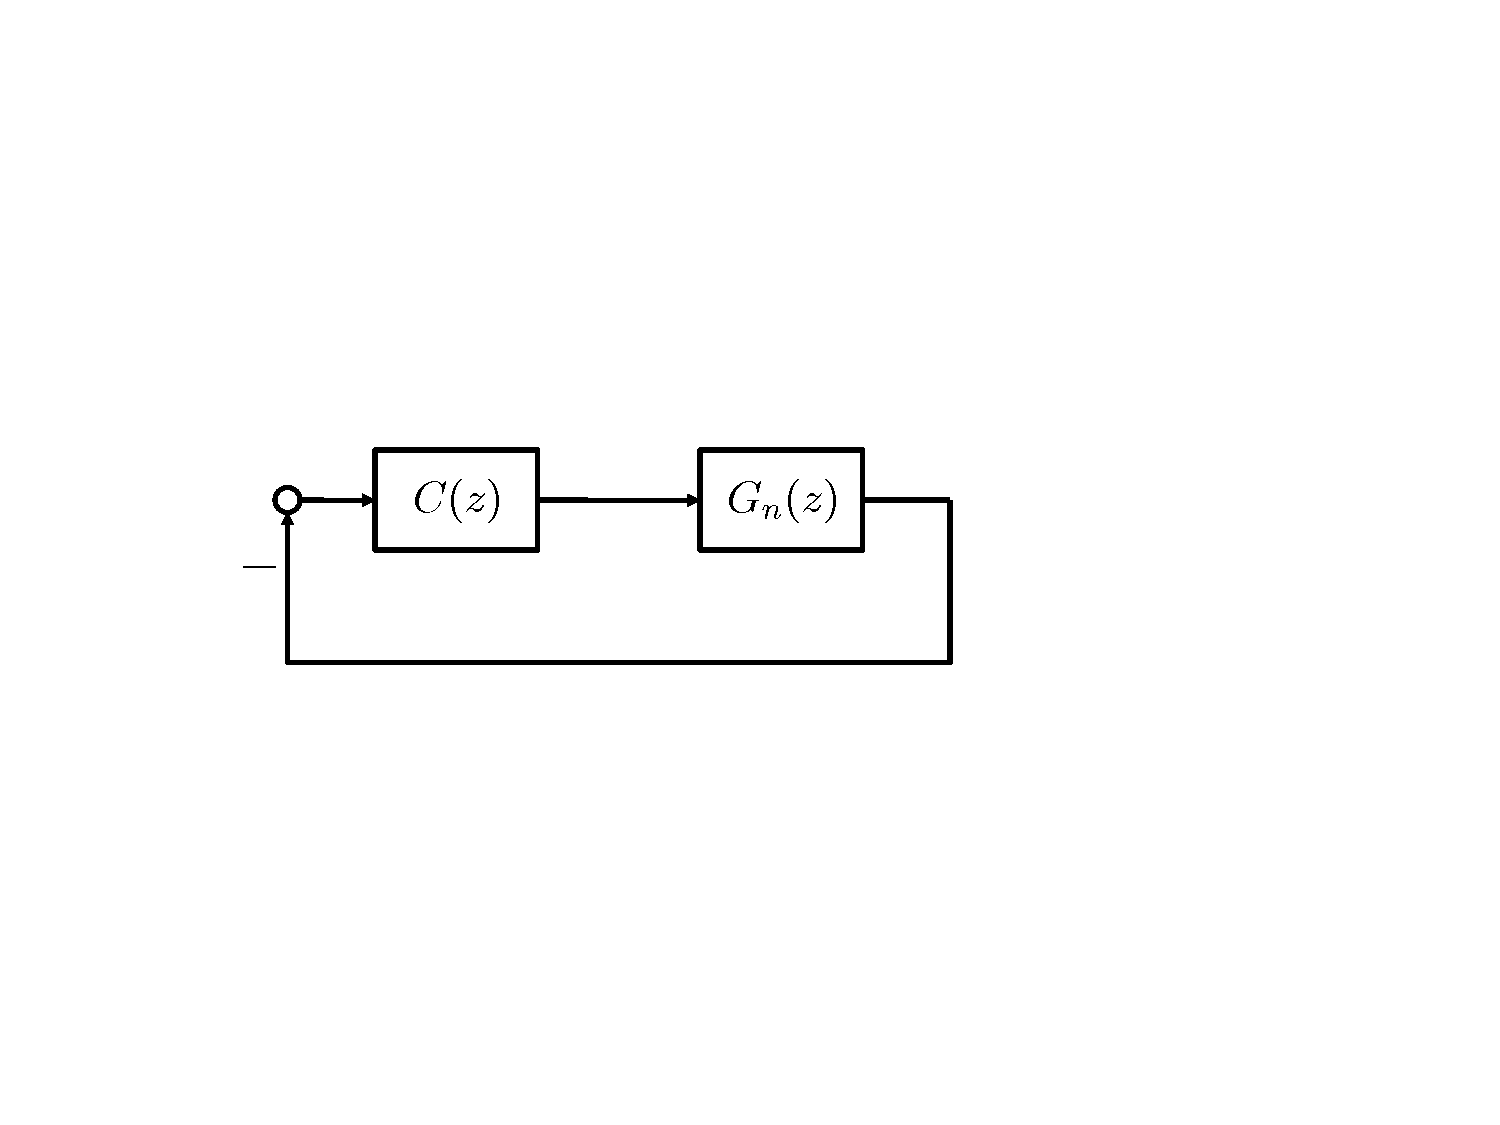
\includegraphics[width=0.3\textwidth]{Disturbance_Observer_multi6}
    \end{figure}
    \pause
    (i.e.\ the \underline{nominal} closed-loop system \underline{without} the disturbance observer is stable)
    \end{enumerate}

\end{frame}

\begin{frame}
    \frametitle{Closed-loop stability}

    We now have the simplified closed-loop system representation
    \begin{figure}
        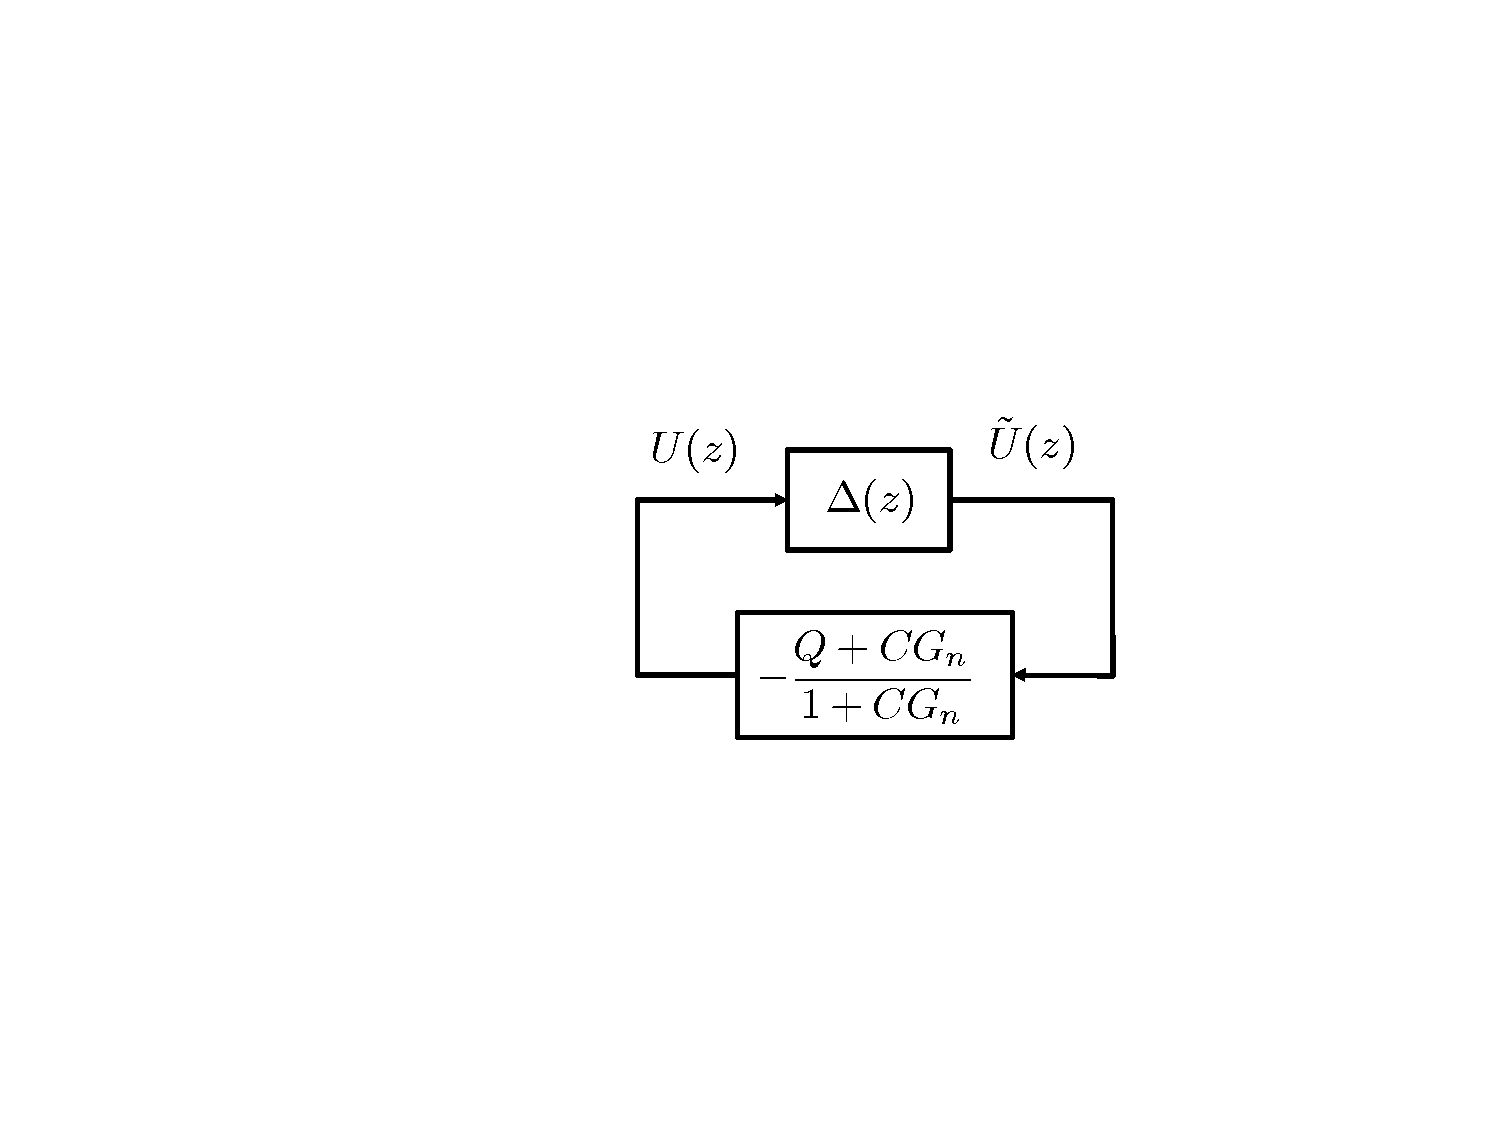
\includegraphics[width=0.3\textwidth]{Disturbance_Observer_multi5}
    \end{figure}
    Using the small-gain theorem, we can therefore guarantee closed-loop stability if:
    \begin{enumerate}
    \item[3.]
    $\displaystyle\left| \frac{Q(\ejw) + C(\ejw) G_n(\ejw)}{1 + C(\ejw) G_n(\ejw) } \right| < \frac{1}{|\Delta(\ejw)|}, \quad \forall \omega \in [0,\pi]$
    \pause
    \newline

    In order to meet this condition, it must be true that $Q(\ejw) \not\approx 1$ whenever $\omega \in [0,\pi]$ is such that $|\Delta(\ejw)| \geq 1$.

    \end{enumerate}

\end{frame}



